\chapter{More Reactor Configurations}\label{ch:appendix-a}

The reactor mass modeling method was demonstrated with a \uox fueled, \codiox
cooled reactor. Three other fuel-coolant configurations were considered for
intergration with the power cycle. The results of these core configurations are
reported here.

For each configuration, 9900 reactivity calculations were performed with
MCNP6.1 and the \keff results were processed using trilinear interpolation with
respect to core radius, fuel fraction, and reflector multiplier. A reflector
optimization for total reactor mass was attempted and an average reflector value
was picked. This value was used to determine the critical core radius as a
function of fuel fraction. Finally, this data was fitted and used in the thermal
hydraulic mass model to constrain the core radius as a function of fuel
fraction.

\section{UW-\codiox}
This configuration is uranium nitride fuel dispersed in a tungsten matrix. The
fuel block is clad with Inconel-718. The
fuel is cooled by supercritical carbon dioxide. A fixed average reflector
multiplier of 0.211 was used for this configuration. Table 



Fig \ref{fig:core_r_un_co2}
shows the critical core radii as a function of fuel fraction.

\begin{figure}[h]
    \centering
    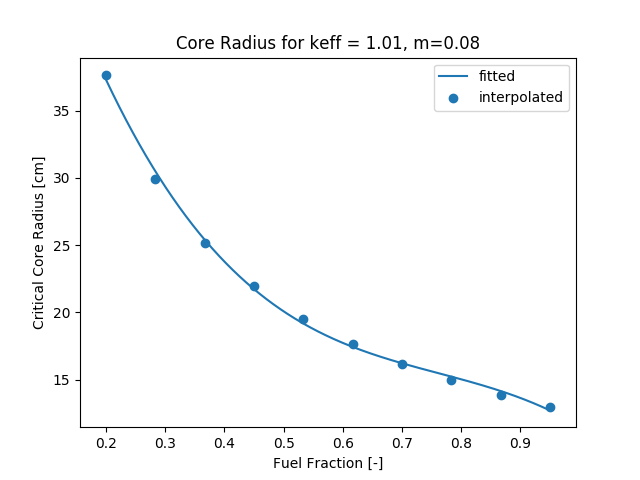
\includegraphics[width=4in]{../images/core_r_un_co2.png}
\caption{Critical core radius for UW-\codiox configuration.}
\label{fig:core_r_un_co2}
\end{figure}

Figure \ref{fig:core_r_un_co2} shows the interpolated core radii and the fitted
curve to the core radii, fuel fraction data. Table \ref{tab:un_co2_fit_coeffs}
contains the 7th order fit coefficients.

\begin{table}[h]
  \centering
  \caption{\uox-\codiox 7th order fit coefficients}
  \begin{tabular}{cc}
    \toprule
     Degree & Coef\\ 
    \midrule                                  
    A$_0$  &  94.223\\
    A$_1$  &  -545.608\\
    A$_2$  &  2009.221\\
    A$_3$  &  -4554.870\\
    A$_4$  &  6393.359\\
    A$_5$  &  -5413.548\\
    A$_6$  &  2530.940\\
    A$_7$  &  -501.210\\
  \end{tabular}
  \label{tab:uo2_co2_fit_coeffs}
\end{table}


\section{\uox-\water}
This configuration is monolithic uranium oxide fuel with Inconel-718 cladding.
The fuel is cooled by supercritical water. A fixed average reflector multiplier
of 0.001 was used for this configuration. The reflector thickness was not
allowed to be zero for modeling convenience in MCNP. The optimization found a
reflector to not be favorable for this configuration. Figure
\ref{fig:core_r_uo2_h2o} shows the critical radius curve, and Table
\ref{tab:uo2_h2o_fit_coeffs} shows the fit coefficients for the 7th order
polynomial fit to the data.

\begin{figure}[h]
    \centering
    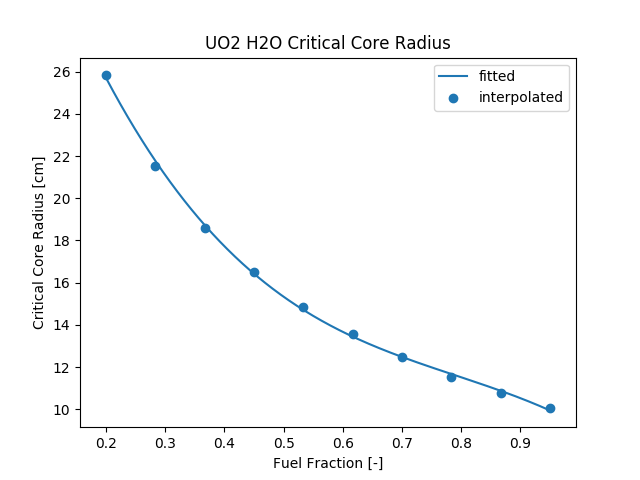
\includegraphics[width=4in]{../images/core_r_uo2_h2o.png}
\caption{Critical core radius for \uox-\water configuration.}
\label{fig:core_r_uo2_h2o}
\end{figure}

\begin{table}[h]
  \centering
  \caption{\uox-\water 7th order fit coefficients}
  \begin{tabular}{cc}
    \toprule
     Degree & Coef\\ 
    \midrule                                  
    A$_0$  &  1\\
    A$_1$  &  1\\
    A$_2$  &  1\\
    A$_3$  &  1\\
    A$_4$  &  1\\
    A$_5$  &  1\\
    A$_6$  &  1\\
    A$_7$  &  1\\
  \end{tabular}
  \label{tab:uo2_h2o_fit_coeffs}
\end{table}



\section{UW-\water}
This configuration is uranium nitride dispersed in a tungsten matrix. The core
is cooled by supercritical \water. A fixed reflector multiplier of 0.0221 was
used for this configuration. Figure \ref{fig:core_r_un_h2o} shows the critical
radius curve, and Table \ref{tab:un_h2o_fit_coeffs} shows the fit coefficients
for the 7th order polynomial fit to the data.

\begin{figure}[h]
    \centering
    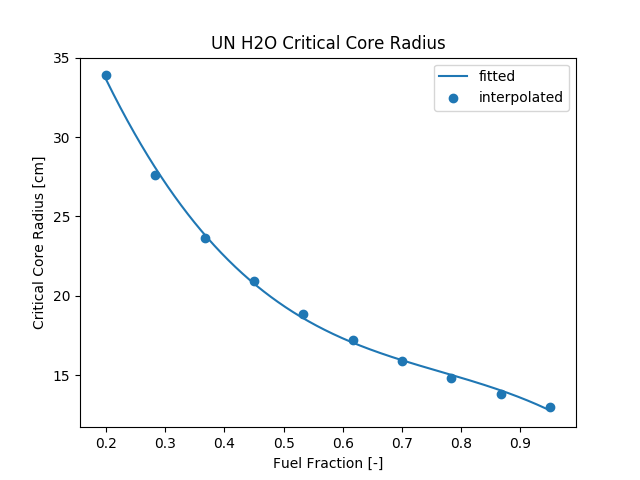
\includegraphics[width=4in]{../images/core_r_un_h2o.png}
\caption{Critical core radius for UW-\water configuration.}
\label{fig:core_r_un_h2o}
\end{figure}


\begin{table}[h]
  \centering
  \caption{UW-\water 7th order fit coefficients}
  \begin{tabular}{cc}
    \toprule
     Degree & Coef\\ 
    \midrule                                  
    A$_0$  &  87.181\\
    A$_1$  &  -509.057\\
    A$_2$  &  1971.832\\
    A$_3$  &  -4736.728\\
    A$_4$  &  7065.368\\
    A$_5$  &  -6372.948\\
    A$_6$  &  3181.888\\
    A$_7$  &  -674.687\\
  \end{tabular}
  \label{tab:un_h2o_fit_coeffs}
\end{table}
